\documentclass{vldb}
\usepackage{pgfplots}
\usepackage{amssymb}
\usepackage{url}
\usepackage{enumitem}
\usepackage[linesnumbered,ruled]{algorithm2e}
\usepackage[export]{adjustbox}
\usepackage{xspace}
\usepackage{breqn}

\newtheorem{example}{Example}
\newtheorem{problem}{Problem}
\newtheorem{definition}{Definition}

\newcommand{\framework}{{\sc GeoGuide}}
\newcommand{\pb}{{\sc GeoGuide}}

\title{GeoGuide: An Interactive Guidance Approach for Spatial Data}

\author{
Behrooz Omidvar-Tehrani$^{\dag}$, Pl\'acido A. Souza Neto$^{\ddag}$\\
\affaddr{
$^{\dag}$The Ohio State University, USA, $^{\ddag}$Federal Institute of Rio Grande do Norte - IFRN, Brazil}\\
\affaddr{
$^{\dag}$\path{omidvar-tehrani.1@osu.edu},
$^{\ddag}$\path{placido.neto@ifrn.edu.br}
}}

\date{}

\begin{document}
\maketitle

\begin{abstract}
spatial data is becoming increasingly available in various domains such as transportation and social science. Discovering patterns and trends in this data provides improved insights for planning and decision making for smart city management, disaster management and other applications. However, exploratory analysis of such data is a challenge due to its huge size and diversity of spatial data. It is often unclear for the analyst {\em what to see next} during an analysis process, i.e., lack of guidance. To tackle this challenge, we formulate guidance as an optimization problem and develop \framework, an efficient interactive guidance approach for spatial data. At each step of an interactive process, $k$-most interesting geographical points become highlighted to guide the analyst through further steps. We illustrate the efficiency and usability of our framework in an extensive set of experiments.
\end{abstract}

\section{Introduction} 
Nowadays, there exists huge amounts of spatial data in various fields of science, such as agriculture, transportation and social science. Analysis of such data is interesting as it is grounded
on reality: each record represents a specific geographical location. Moreover, understanding patterns and trends provides insights leading to improved user planning and decision making. Some instance applications of spatial data are smart city management, disaster management and autonomous transport.
% \cite{RoddickEHPS04,Telang:2012}.

\begin{figure}[t]
  \centering
  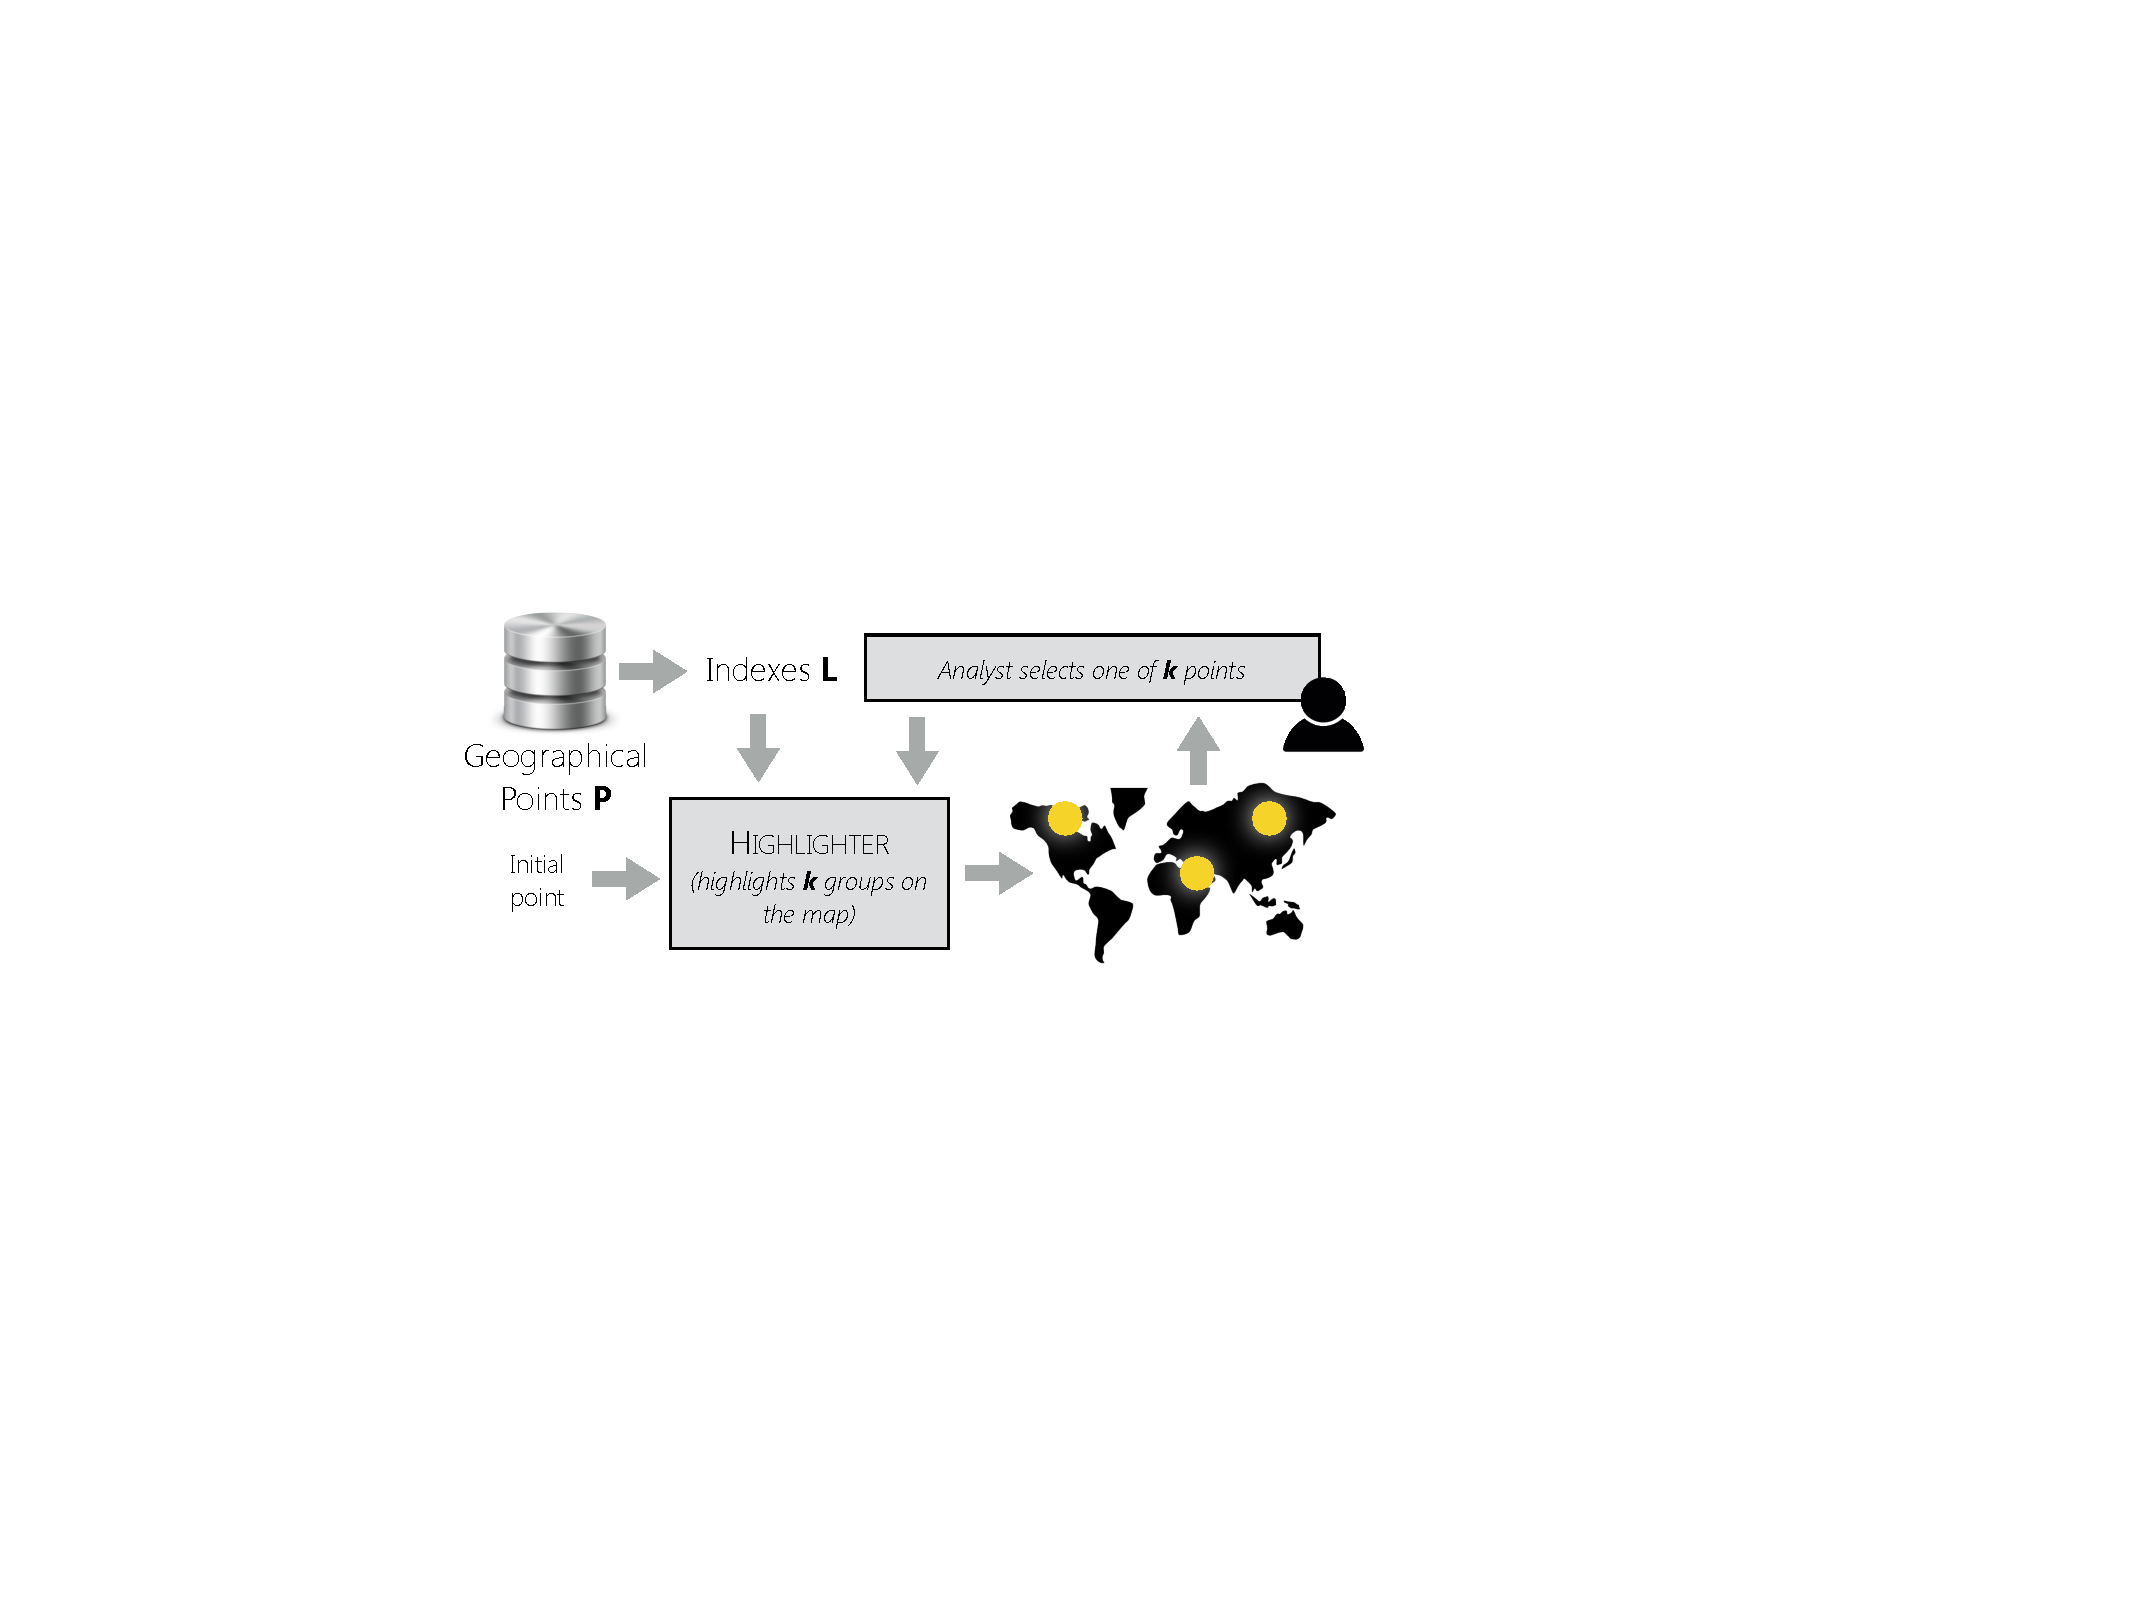
\includegraphics[width=\columnwidth]{figs/framework}
\caption{\framework\ Framework}
\label{fig:framework}
\vspace{-10pt}
\end{figure}

Spatial data analysis is often performed in {\em exploratory context}: the analyst does not have a precise query in mind and she explores data in iterative steps in order to find potentially interesting results. Traditionally, an exploratory analysis scenario on spatial data is described as follows: the analyst visualizes a subset of data using a query in an off-the-shelf product (e.g., Tableau\footnote{\it http://www.tableau.com},
% Exhibit\footnote{\it http://www.simile-widgets.org/exhibit/},
Spotfire\footnote{\it http://spotfire.tibco.com}). The result will be illustrated on a geographical map. Then she investigates on different parts of the visualization by zooming in/out and panning the map in order to discover patterns and trends of interest. The analyst may iterate on this process several times by issuing different queries and focusing on different aspects of data. 

The literature in spatial data analysis has a focus on {\em efficiency} of exploratory iterations: {\em ``how can analysts navigate in spatial data fluidly?''} The common approach is to design pre-computed indexes which enable efficient retrieval of spatial data (e.g., \cite{lins2013nanocubes}). However, there has been fewer attention to the {\em value} of spatial data. Despite the huge progress on efficiency front, an analyst may easily get lost in the plethora of geographical points because $i.$ she doesn't know what to investigate next in an exploratory context and $ii.$ she may get distracted and miss interesting points by visual clutter caused by huge point overlaps. In other words, although iteration transitions (between one analysis step to the other) can be performed efficiently, the decision which forms a transition, remains unclear. The following example illustrates the challenge in practice.

\begin{example}
\label{ex:airbnb}
Liam is planning a short trip to Paris. He decides to rent a home-stay from Airbnb website\footnote{\it http://www.airbnb.com}. He is open to any type of lodging and he wants to explore different options (i.e., exploratory analysis). He queries all available locations in Paris with a fair price. His query results in 3000 locations. As he has no other preferences, an exhaustive investigation needs scanning each location independently which is nearly infeasible. In case he wants to focus on a smaller set of options, it is not clear which subset he needs to look at. While he is looking at primary locations in the list, he shows interest in having ``balcony'' as amenity and being close to Eiffel tower. An ideal system can capture this feedback in order to short-list a small subset of remaining locations that Liam should consider as high priority.
\end{example}

To overcome the challenge of value in exploratory analysis, visualization environments offer a complete tool-set to manipulate data (filter, aggregate, etc.). In practice, this duplicates the problem: the analyst is left alone in a huge space of spatial data and tools. The principled challenge for the analyst is {\em ``what to see next''} in the exploratory context. A {\em guidance} mechanism is then necessary to point out potential future directions of analysis.

In this demo paper, we introduce \framework, an interactive framework to highlight a subset of geographical points based on analyst feedback. The highlighted set facilitates the decision-making process by providing guidance on what the analyst should potentially concentrate on. The set of highlights is deliberated over high quality. We consider two quality metrics in \framework: {\em relevance} and {\em diversity}. First, each highlighted point should be relevant to historical choices of the analyst. Second, highlights should be geographically diverse to unveil different aspects of analysis. Both quality metrics are interdependent to compute the set of highlights.

The literature contains several instances of feedback exploitation to guide the analyst in further analysis steps (e.g., \cite{boley2013one}). The common approach is a top-$k$ processing methodology in order to prune the search space based on the explicit feedback and recommend a small subset of interesting results of size~$k$. A clear distinction of \framework\ is that it doesn't aim for pruning, but leveraging the actual data with potential interesting results that the analyst may miss due to the huge volume of spatial data. While in top-$k$ processing algorithms, analyst choices are limited to $k$, \framework\ has a freedom of choice where highlights get seamlessly updated with new analyst choices. The following example describes an application of \framework\ in business domain.

\begin{example}
\label{ex:flight}
Tiffany is a data scientist and is tasked to design a ``chain marketing'' strategy for a Peking Duck product (a Chinese duck dish). She decides to exploit Yelp data\footnote{\it https://www.yelp.com/} (i.e., restaurant check-ins) to find out the advertisement chain. She performs her analysis in \framework. In the first step, she shows interest towards New York region, where the headquarters of the company is located and the product has already gained success. The system will then provide few highlights in diverse regions: San Fransisco, Washington DC and Marlton, NJ. All regions seem interesting to Tiffany as they exhibit similar eating profile with New York, hence potentials for chaining the advertisement. She decides to pick Marlton due to its proximity so that she can reduce transportation costs. The system will then provide other highlights based on her updated feedback. She can then make the city-to-city chain marketing strategy in iterative steps using highlights.
\end{example}

There exist few instances of information-highlighting methods in the literature \cite{Liang2010,Robinson2011,wongsuphasawat2016voyager,willett2007scented}. However all these methods are {\em objective} and do not apply to the context of spatial guidance where user feedback is involved.  In terms of recommendation, few approaches focus on spatial dimension \cite{Bao2015,Levandoski:2012} while the context and result diversification are missing.

\section{GeoHighlight Framework}
\label{sec:pb}
In this section, we describe the functionality of \framework\ which is an inspiration from both recommendation \cite{Omidvar-Tehrani:2015} and visual highlighting \cite{Liang2010,Robinson2011} methodologies. The aim of this framework is to guide analysts in large-scale spatial data analysis. We follow a highlighting strategy where we stress out regions of interest based on analyst historical choices (i.e., feedback).

In our framework, we consider a spatial database ${\cal D}$ consisting $\langle {\cal P}, {\cal A} \rangle$ where ${\cal P}$ is the set of
geographical points and ${\cal A}$ is the set of point attributes. For each $p \in {\cal P}$, we consider a tuple $\langle lat, lon, alt\rangle$ which denotes $p$'s geographical coordinates (latitude, longitude and altitude respectively). The set ${\cal A}_p$ contains attribute-values for $p$ over the schema of ${\cal A}$. For instance, on a bike-sharing dataset, ${\cal A}_p = \langle${\tt female}, {\tt young}, {\tt hybrid-bike}$\rangle$ on the schema ${\cal A} = \langle${\tt gender}, {\tt age}, {\tt type}$\rangle$ denotes that $p$ is associated to a young female cyclist who rides a hybrid bike. The set ${\cal A}$ is domain-dependent and defines the semantics of a spatial dataset.

We also define a feedback vector ${\cal F}$ on the schema ${\cal A}$ initialized by zero. The vector gets updated by ${\cal A}_p$ whenever the analyst shows interest in a geographical point $p$. Feedback vector is always kept normalized where $\Sigma_{v \in {\cal F}}(v) = 1.0$. Unlike the literature which mainly focuses on explicit feedback (where the analyst should clearly reflect her likes and dislikes), we investigate on implicit feedback. This enables the system to capture {\em what the analyst may miss} instead of what the analyst has clearly investigated before. We consider two different ways to capture implicit feedback.

\begin{itemize}[leftmargin=*]
\item {\bf Gaze.} During spatial data analysis, it is often the case analysts look at some regions of interest but forget to provide an explicit feedback. For instance in Example \ref{ex:airbnb}, while Liam is focusing on home-stays close to the Eiffel tower, he also looks at farther locations with easy train access. However, he never clicks on them. We call this latent signal, {\em gaze}. Gaze can be captured by tracking the directions of analyst looking. It can be done for example by http://www.xlabsgaze.com/. Also we can imitate by cursor tracking.
\item {\bf Session Time.} In most spatial datasets, there is profile page dedicated to each point. For instance restaurant pages in Yelp. We measure the amount of time that the user takes in a page as implicit feedback. For instance, if the user looks a lot at Indian page, then it seems that he is interested in this type of resturants.
\end{itemize}

At each step of the analysis, \framework\ highlights few points based on the ${\cal F}$ content. The decision is made based on two quality metrics, i.e., relevance and diversity. 

\vspace{5pt}
\noindent {\bf Relevance.} Highlights should be in the same line with previous choices of the analyst. Note that we consider {\em contextual-based} relevance and not {\em distance-based} relevance. The reason originates from our data observation. For instance in a taxi dataset, consider a ride in New York for a young male customer for an itinerary of 10 kilometers and \$3 tip. In contrary to thousands of kilometers of geographical distance, the ride is very relevant to another one in San Fransisco for a middle-age male customer for an itinerary of 8 kilometers and \$2.5 tip.

The relevance between a point $p$ and the feedback vector ${\cal F}$ is defined as follows.

% \begin{definition}[Relevance]
% Given two points $p$ and $p'$ and their attribute values ${\cal A}_{p}$ and ${\cal A}_{p'}$, the relevance between $p$ and $p'$ is a value between $0$ and $1$ denoted as $\mathit{relevance}(p,p') = \mathit{average}_{a \in {\cal A}_{p} \cup {\cal A}_{p'}}(\mathit{sim({\cal A}_{p}, {\cal A}_{p'}, a)})$.
% \label{def:rel}
% \end{definition}

\begin{dmath}
\label{eq:rel}
\mathit{relevance}(p,{\cal F}) = \mathit{average}_{a \in {\cal A}_{p} \cap {\cal F}}(\mathit{sim(p, {\cal F}, a)})
\end{dmath}

The similarity function $\mathit{sim}()$ can be any function such as Jaccard and Cosine. Each attribute can have its own similarity function (as string and integer attributes are compared differently.) Then $\mathit{sim}()$ works as an overriding-function which provides encapsulated similarity computations for any type of attribute.

The point-feedback relevance is neither monotonic nor anti-monotonic. In other words, a highly relevant point to the feedback vector at step $i$ may become totally irrelevant to the updated feedback vector at step $i+1$. The reason is the dynamic nature of the feedback vector which may drastically evolve at each analysis step. For efficiency reasons, we employ a static component and build indexes which capture point-point relevance to speed up online computations.

\vspace{5pt}
\noindent {\bf Diversity.} Highlighted points should also represent distinct regions so that the analyst can observe different aspects of data and decide based on the big picture. Given a set of points $s = \{ p_1, p_2 \dots \}$, we define {\em diversity} as follows.

\begin{dmath}
\label{eq:divs}
\mathit{diversity}(s) = \mathit{average}_{\{p, p'\} \subseteq s | p \neq p' } \mathit{distance}(p,p')
\end{dmath} 

The function $\mathit{distance}(p,p')$ operates on geographical coordinates of $p$ and $p'$ and can be considered as any distance function of Chebyshev distance family such as Eucledian. However, as distance computations are done in {\em spherical space} using latitude, longitude and altitude, it is au-naturel to employ Harvestine distance shown in Equation \ref{eq:harvestine}.

\begin{dmath}
\label{eq:harvestine}
distance(p,p') = [ acos(cos(p_{lat}) . cos(p'_{lat}) . cos(p_{lon}) . cos(p'_{lon})\\ + cos(p_{lat}) . sin(p'_{lat}). cos(p_{lon}) . sin(p'_{lon}) + sin(p_{lat}) . sin(p'_{lat})) ] \times earth\_radius
\end{dmath}

% \vspace{5pt}
% Following aforementioned desiderata, we formulate highlighting as an optimization-based problem on relevance and diversity dimensions.

% \begin{problem}[\pb]
% \label{pb:geoh}
% Given an input point $p$ and a threshold $\sigma$, the problem is to return top-$k$
%  points denoted $S_p$ where $|S_p| = k$ and $\forall p' \in S_p, \mathit{relevance}(p,p') \geq \sigma$ and $\mathit{diversity}(S_p)$ is maximized.
% \end{problem}

% Problem \ref{pb:geoh} is hard due to the huge space of spatiotemporal data: for any given point $p$, an exhaustive search over all other points is necessary to find $k$ points with maximal relevance. Moreover, the problem investigates in two dimensions at the same time (relevance and diversity) which makes it more challenging.

 \framework\ requires an efficient algorithm for dynamically analyzing and comparing geographical points (Figure \ref{fig:framework}). Although \framework\ operates on points, its functionality can be easily extended to regions using point-clustering methods such as $k$-means. Intuitively, \framework\ is a layer on top of raw visualization which highlights representatives at each analysis iteration. The representatives reflect the feedback of the analyst in previous steps.

 \framework\ operates in two steps: {\sc Preparation} and {\sc Highlighter}. In order to speed up computing relevance in online execution, we pre-compute an inverted index for each single geographical point in ${\cal P}$ in the offline {\sc Preparation} step (as is commonly done in Web search). Each index ${\cal L}_p$ for the point $p$ stores all other points in ${\cal P}$ in decreasing order of their relevance with $p$. Thanks to the parameter $\sigma$, we only partially materialize the indexes.

 Algorithm \ref{algo:geoh} illustrates the online execution step of \framework\, so called {\sc Highlighter}. The algorithm is a single greedy procedure that solves the \pb\ problem. {\sc Highlighter} is called at each interactive step of \framework\ (as in Figure \ref{fig:framework}). The algorithm admits as input a point $p \in {\cal P}$ and returns the best $k$ points denoted ${\cal S}_p$.

To comply with the desiderata {\bf D5}, we consider a time limit parameter $tlimit$ in Algorithm \ref{algo:geoh}. In a {\em best-effort} strategy, the algorithm bounds user waiting time by $tlimit$ to return the best possible results by then.

\begin{algorithm}[t]
\DontPrintSemicolon
\KwIn{$p \in {\cal P}$, $\sigma$, $k$, $tlimit$}
% \KwOut{${\cal S}_p$}
${\cal S}_p \gets get\_top\_k(\mathit{{\cal L}^p})$\;\label{cd:gettopk}
$p_{next} \gets get\_next(\mathit{{\cal L}^p})$\;\label{cd:getnext}
\While{$(tlimit$ $not$ $exceeded \wedge relevance(p,p_{next}) \geq \sigma)$}{\label{cd:beginwhile}
\For{$p_{current} \in {\cal S}_p$}{
\If{$\mathit{diversity\_improved}({\cal S}_p,p_{next},p_{current})$}{\label{cd:betterdiv}
${\cal S}_p \gets \mathit{replace}({\cal S}_p,p_{next},p_{current})$\;
$break$\;
}
}
$p_{next} \gets get\_next({\cal L}^p)$\;}\label{cd:endwhile}
\Return{${\cal S}_p$}\; 
\caption{{\sc Highlighter} Algorithm}
\label{algo:geoh}
\end{algorithm}
% \vspace{-10pt}
% behrooz: mention working of sacrification

{\sc Highlighter} begins by retrieving the most relevant points to $p$ by simply retrieving the $k$ highest ranking points in ${\cal L}_p$ (line \ref{cd:gettopk}). Function $get\_next({\cal L}_p)$ (Line \ref{cd:getnext}) returns the next point $p_{next}$ in ${\cal L}_p$ in sequential order. Lines \ref{cd:beginwhile} to \ref{cd:endwhile} iterate over the inverted indexes to determine if other points should be considered to increase diversity while staying within the time limit and not violating the relevance threshold with the selected point. Since points in ${\cal L}_g$ are sorted on decreasing relevance with $p$, the algorithm can safely stop as soon as the relevance condition is violated (or if the time limit is exceeded).

The algorithm then looks for a candidate point $p_{current} \in {\cal S}_p$ to replace in order to increase diversity. The boolean function $\mathit{diversity\_improved}()$ (line \ref{cd:betterdiv}) checks if by replacing $p_{current}$ by $p_{next}$ in ${\cal S}_p$, the overall diversity of the new ${\cal S}_p$ increases.

% \vspace{5pt}
% \noindent {\bf Complexity Analysis.} The number of diversity improvement loops (lines \ref{cd:beginwhile} to \ref{cd:endwhile}) is $|{\cal L}_p| = |{\cal P}|$ in worst case. For each point $g_{current} \in {\cal S}_p$, we verify if the diversity score is improved by $\mathit{diversity\_improved}()$, hence $\mathcal{O}(k^2$). The time complexity of the algorithm is then $\mathcal{O}(k^2.|{\cal P}|)$.


At each iteration, the feedback vector is compared with all points to find the ones which are more similar to analyst feedback. To speed up comparison, we exploit boolean representations. We convert both the feedback and point identity to booleans and make boolean comparisons which are indeed faster.

We dont want to be slow in price of values and insights. So we make our algorithm best effort and bound it to a time limit. In time limit, it starts from most similar options only to previous options and they also become diverse.

We evaluate the efficiency and usefulness of \framework\ in an extensive set of experiments. We consider two types of experiments: first, a performance study measures the influence of relevance and size constraint thresholds on execution time. Second, we measure the usefulness of our framework in a user study.

\vspace{5pt}
\noindent {\bf Experiment Settings.} Unless otherwise stated, we use the same settings discussed in Section \ref{sec:scenarios}. All experiments are implemented in Python (functionality) and JavaScript D3 (visualization) on a 2.8GHz Intel Core i5 machine with an 16GB main memory, running OS X 10.9.2.

\begin{figure}
 \centering
 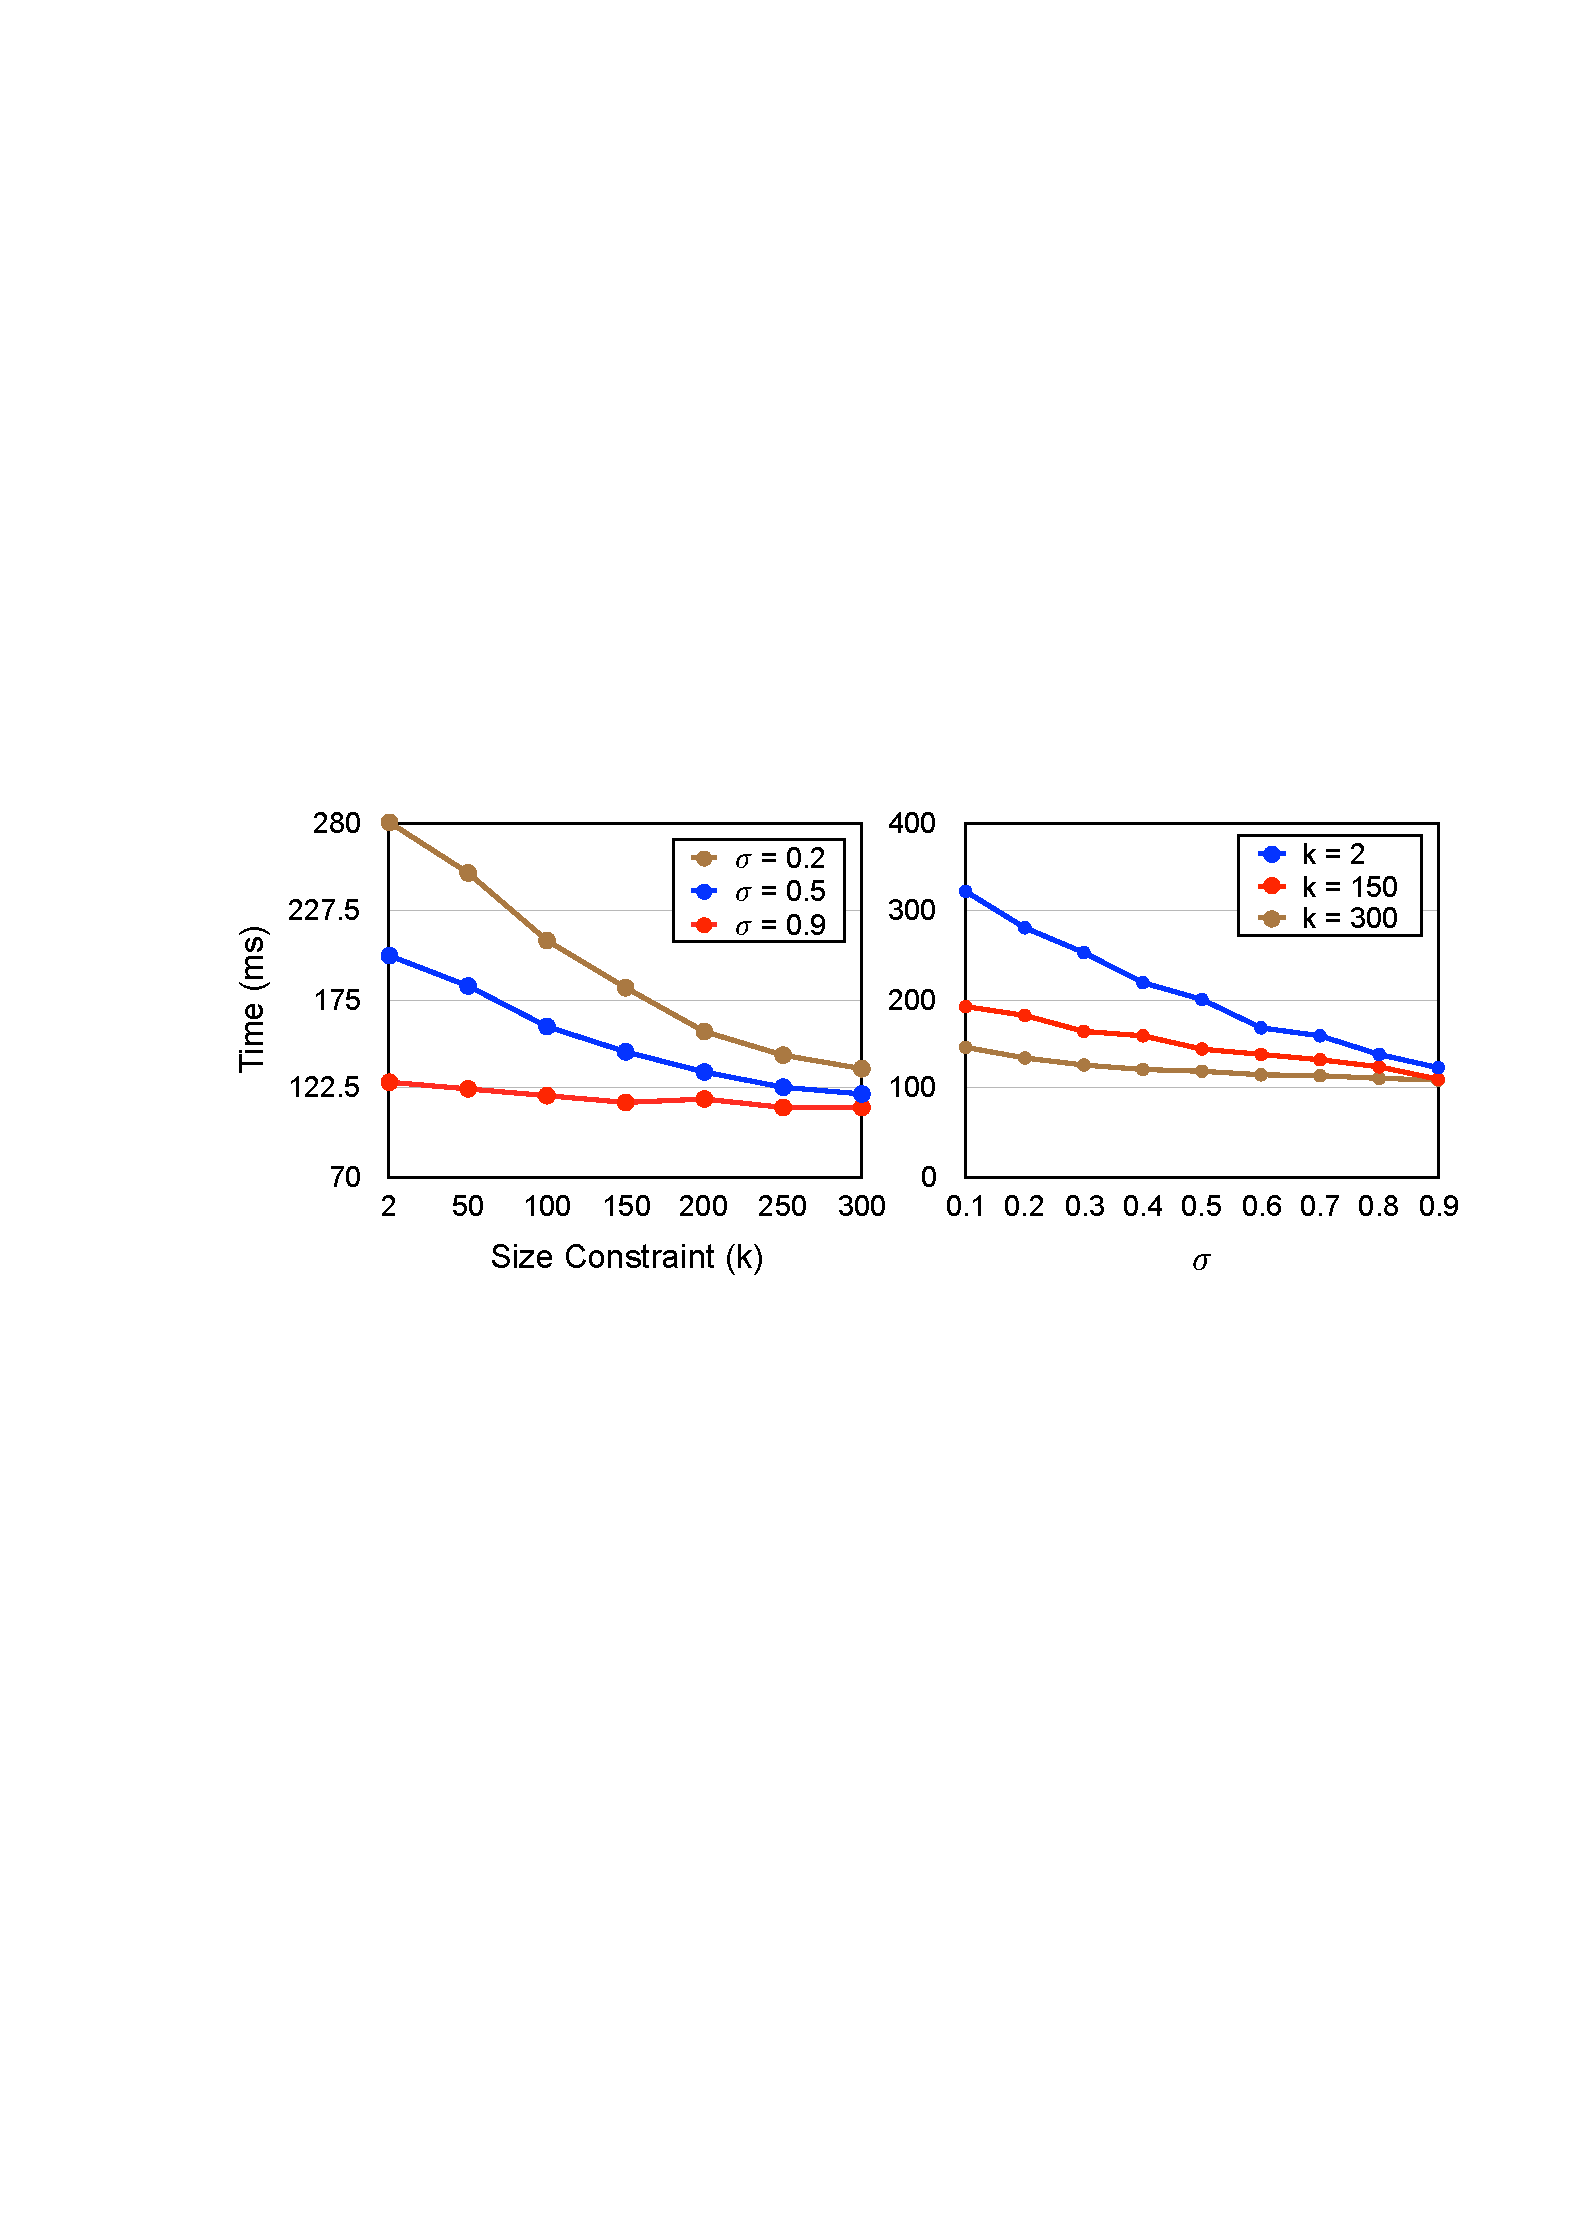
\includegraphics[width=\columnwidth]{figs/performance}
\caption{Performance Evaluation}
\vspace{-10pt}
\label{fig:performance}
\end{figure}

% \begin{figure}
%   \centering

% % Preamble: 
% \pgfplotsset{width=\columnwidth,compat=1.13}
% \tiny
% \begin{minipage}[b]{0.45\linewidth}
% \begin{tikzpicture}
% \begin{axis}[
% 	xlabel={Size Constraint (k)},
% 	ylabel={Similarity}
% ]

% \addplot table [x=k, y=sim, col sep=comma] {figs/charts/c01/02.csv};
% \addplot table [x=k, y=sim, col sep=comma] {figs/charts/c01/05.csv};
% \addplot table [x=k, y=sim, col sep=comma] {figs/charts/c01/07.csv};
% \addplot table [x=k, y=sim, col sep=comma] {figs/charts/c01/09.csv};

% \tiny
% %\legend{$\sigma=0.2$, $\sigma=0.5$, $\sigma=0.9$}
% \end{axis}
% \end{tikzpicture}
% \end{minipage}
% \hspace{0.2cm}
% \begin{minipage}[b]{0.45\linewidth}
% \begin{tikzpicture}
% \begin{axis}[
% 	xlabel={Size Constraint (k)},
% 	ylabel={Diversity}
% ]

% \addplot table [x=k, y=div, col sep=comma] {figs/charts/c01/02.csv};
% \addplot table [x=k, y=div, col sep=comma] {figs/charts/c01/05.csv};
% \addplot table [x=k, y=div, col sep=comma] {figs/charts/c01/07.csv};
% \addplot table [x=k, y=div, col sep=comma] {figs/charts/c01/09.csv};
% \tiny
% %\legend{$\sigma=0.2$, $\sigma=0.5$, $\sigma=0.9$}
% \end{axis}
% \end{tikzpicture}
% \end{minipage}

% %%% SECOND LINE %%% 
% \bigskip

% \begin{minipage}[b]{0.45\linewidth}
% \begin{tikzpicture}
% \begin{axis}[
% 	%legend pos=outer north east,
% 	xlabel={Size Constraint (k)},
% 	ylabel={Time(sec)}
% ]

% \addplot table [x=k, y=0.2, col sep=comma] {figs/charts/fig3.csv};
% \addplot table [x=k, y=0.5, col sep=comma] {figs/charts/fig3.csv};
% \addplot table [x=k, y=0.7, col sep=comma] {figs/charts/fig3.csv};
% \addplot table [x=k, y=0.9, col sep=comma] {figs/charts/fig3.csv};
% \tiny
% %\legend{$\sigma=0.2$,$\sigma=0.5$,$\sigma=0.7$,$\sigma=0.9$}
% \end{axis}
% \end{tikzpicture}
% \end{minipage}
% \hspace{0.2cm}
% \begin{minipage}[b]{0.45\linewidth}
% \begin{tikzpicture}
% \begin{axis}[
% 	%legend pos=outer north east,
% 	xlabel={Sigma ($\sigma$)},
% 	ylabel={Time(sec)}
% ]

% \addplot table [x=sigma, y=2, col sep=comma] {figs/charts/fig4.csv};
% \addplot table [x=sigma, y=100, col sep=comma] {figs/charts/fig4.csv};
% \addplot table [x=sigma, y=200, col sep=comma] {figs/charts/fig4.csv};
% \addplot table [x=sigma, y=300, col sep=comma] {figs/charts/fig4.csv};

% \tiny
% %\legend{$k=2$,$k=100$,$k=300$,$k=300$}
% \end{axis}
% \end{tikzpicture}
% \end{minipage} 
%   \caption{Performance Evaluation}
% \vspace{-10pt}
% \label{fig:performance}
% \end{figure}

% \newpage
% \vspace{-20pt}
\noindent {\bf Performance Study.} \framework\ is designed for exploratory context where interactivity is a need. The ``best-effort'' greedy approach of {\sc Highlighter} (Algorithm \ref{algo:geoh}) guarantees to return the best possible results within a time limit. We consider a large time limit ($tlimit = 2s$) in order to evaluate the effect of relevance and size constraint thresholds on execution time.
% Figure \ref{fig:performance} illustrates the results by measuring the execution time.

Figure \ref{fig:performance} left illustrates the effect of size constraint by varying $k$ from $2$ to $300$. In general, larger values of $\sigma$ provides more freedom for the algorithm hence more time-consuming. An interesting observation is that increasing $k$ leads decreasing execution time. This is because in larger sets, there exist fewer opportunities for increasing diversity, hence {\sc Highlighter} terminates early.

Figure \ref{fig:performance} right confirms that lower values of $\sigma$ decreases execution time as they provide more flexibility for diversity improvement. For larger values of $k$ (i.e., when $k >100$), the influence of $\sigma$ on execution time becomes insignificant.

\vspace{5pt}
\noindent {\bf User Study.}
The principled question that we ask ourselves is whether \framework\ is useful for analysts in practice. To answer this question, we designed a user study with $24$ participants (students in Computer Science). Half of the participants know the New York region well (experts) and the other half have a limited knowledge (novice). In our user study, we define a task for each participant and ask him/her to fulfill the task using both \framework\ and {\sc Tableau} (as the most advanced spatiotemporal visualization tool). Then we measure the cardinality of steps to reach the goal.

We define two tasks, {\em T1: finding a point in a requested location}, and {\em T2: finding a point with a requested profile}. As an example for {\em T1}, we ask participants to find points in the Central Park area. An example of {\em T2} is to find a drop-off point with \$2 tip whose trip distance is 3 kilometers. Participants may begin their navigation from three different starting points: {\em I1: close to the goal}, {\em I2: far from the goal}, and {\em I3: random}. We evaluate the effect of expertise, goal and starting point on the analysis length. Figure \ref{fig:userstudy} illustrates the results for novice (left) and expert (right) participant.

We observe that in general, it takes in average 10.7 steps to reach a defined goal in \framework, i.e., 33 steps less than {\sc Tableau}. This shows that the guidance component helps analysts discover their data and quickly reach to the goal. Level of expertise improves the analysis length in average by 4 steps. Interestingly, starting points do not have a huge influence. It is potentially due to the diversity component which provides distinct options. We also observe that {\em T2} is an easier task than {\em T1}. This is potentially due to similarity component where the analyst can request options similar to what she has already seen and greedily moves to match profiles.

\begin{figure}[t]
 \centering
 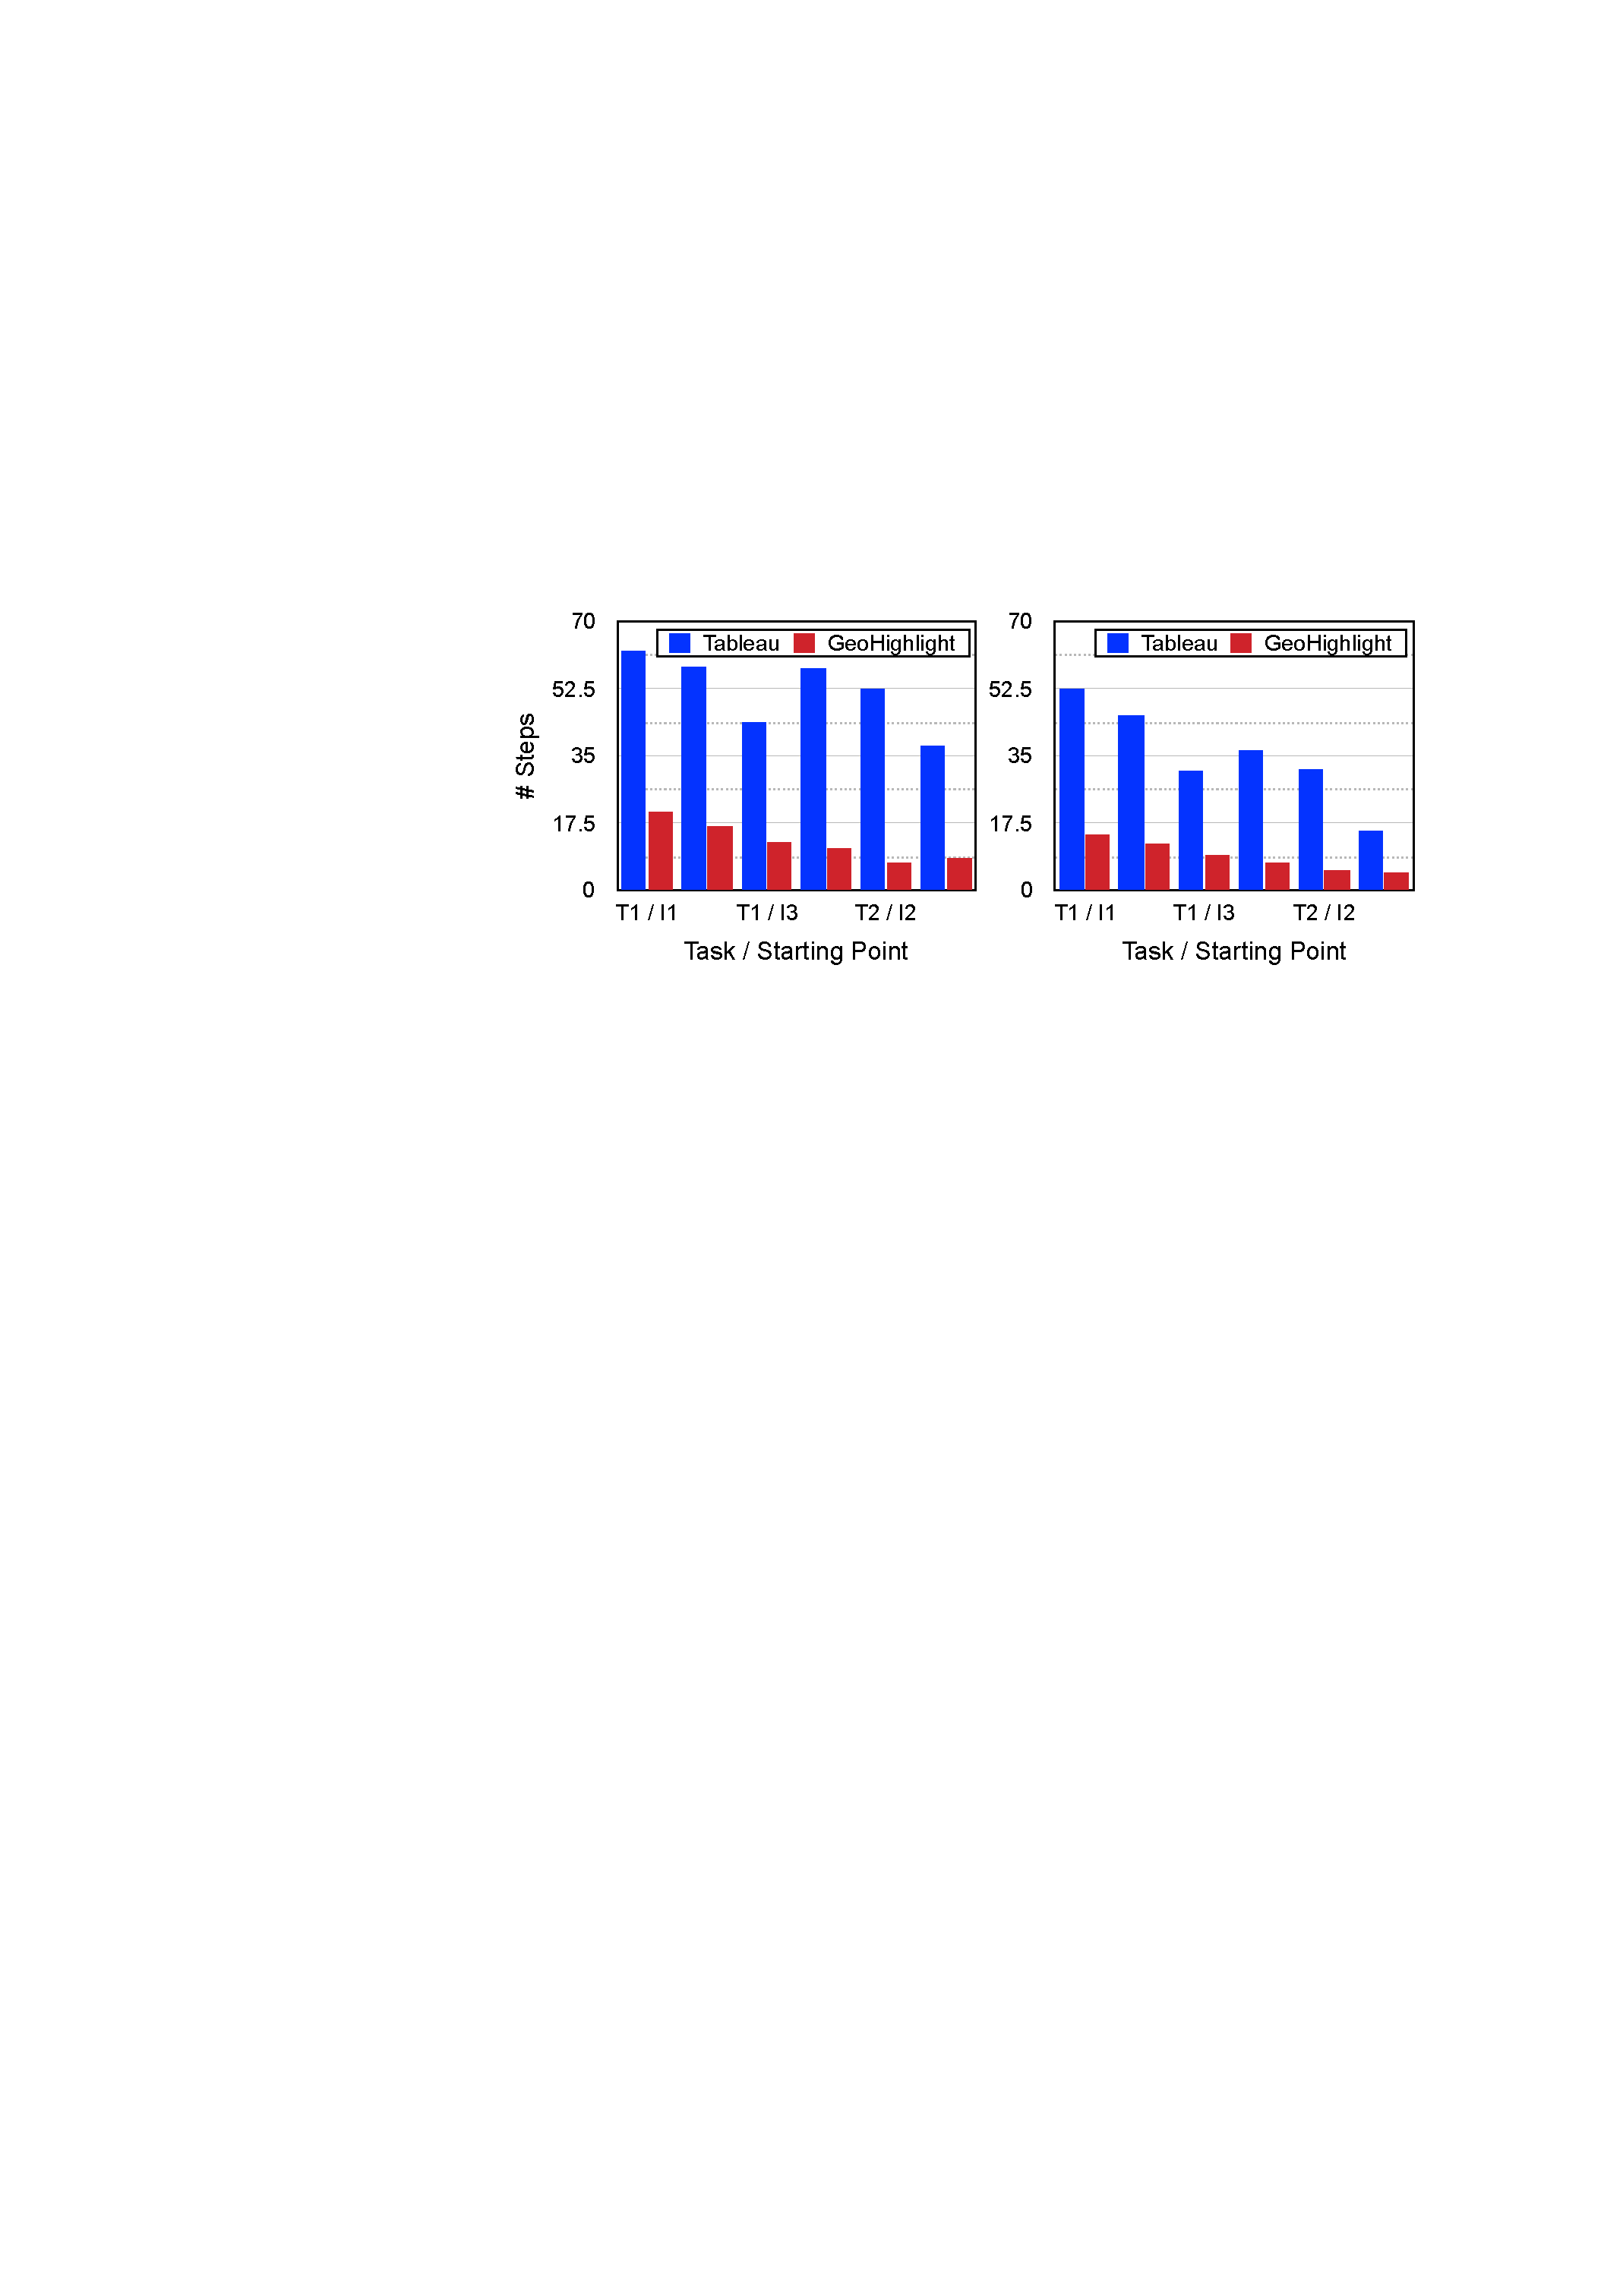
\includegraphics[width=\columnwidth]{figs/userstudy}
\caption{User Study}
\vspace{-5pt}
\label{fig:userstudy}
\end{figure}


% We also asked our participants about their insights on \framework. We ask them to rate the following metric on a 5-star scale: {\em usefulness} and {\em ease-of-use}. In summary, we found that \colorred{[explain received results]}.

\section{Demonstration Plan}
Demonstration attendees can participate as analysts in \framework. We provide several spatial datasets in our demo session: $i.$ Yelp dataset for restaurant check-ins with 229,907 points and 11,537 attribute-values, $ii.$ Airbnb dataset for short-term lodging with 4,200,000 points and 2000 attribute-values, $iii.$ New York taxi dataset with 173,179,759 points and 18 attribute-values, and $iv.$ New York bike-sharing dataset with XXX points and XXX attribute values. We describe three demonstration scenarios as follows.

\vspace{5pt}
\noindent{\bf Scenario 1.} We demonstrate on New York taxi dataset how \framework\ can contribute to urban planning and fleet management. We consider an explicit goal of discovering which neighborhoods work the best for which drivers to increase the overall availability of taxis in the city. We show how a chain of cab stations can be picked by \framework\ to increase availability.

\vspace{5pt}
\noindent{\bf Scenario 2.} We demonstrate on Airbnb dataset how \framework\ can contribute to approach a lodging of interest based on analyst's feedback. The attendee will observe that he/she can quickly reach to satisfying housing solutions based her previous selections. We consider the concrete case of finding a cheap lodging solution near Eiffel tower which seems infeasible.

\vspace{5pt}
\noindent{\bf Scenario 3.} We demonstrate on Yelp dataset how \framework\ can contribute to reach an early consensus on a restaurant. The attendee will observe that his/her preferences will be immediately captured and reflected in future highlights.


% We illustrate an application of \framework\ in a realistic scenario for New York taxi dataset\footnote{\it https://data.cityofnewyork.us/view/gn7m-em8n}. This dataset has been frequently exploited for urban analysis
% % \cite{ferreira2013visual,DBLP:journals/debu/FreireCVZ16}.
% (e.g. in \cite{DBLP:journals/debu/FreireCVZ16}).
% The dataset contains 173,179,759 records of taxi trips and 18 attributes such as pickup and dropoff date/time, passenger count and trip distance.
% The dataset size is 27.9 GB with informations of trips from 2014.
% The scenario illustrates how an analyst can achieve an exploratory analysis goal. We preprocessed the original dataset and considered a subset of 20K unique points for the sake of clarity of results. We employ {\sc Highlighter} (Algorithm \ref{algo:geoh}) with following parameters: $\sigma = 0.2$, $k = 5$ and $tlimit = 200ms$.

\begin{figure}
  \centering
  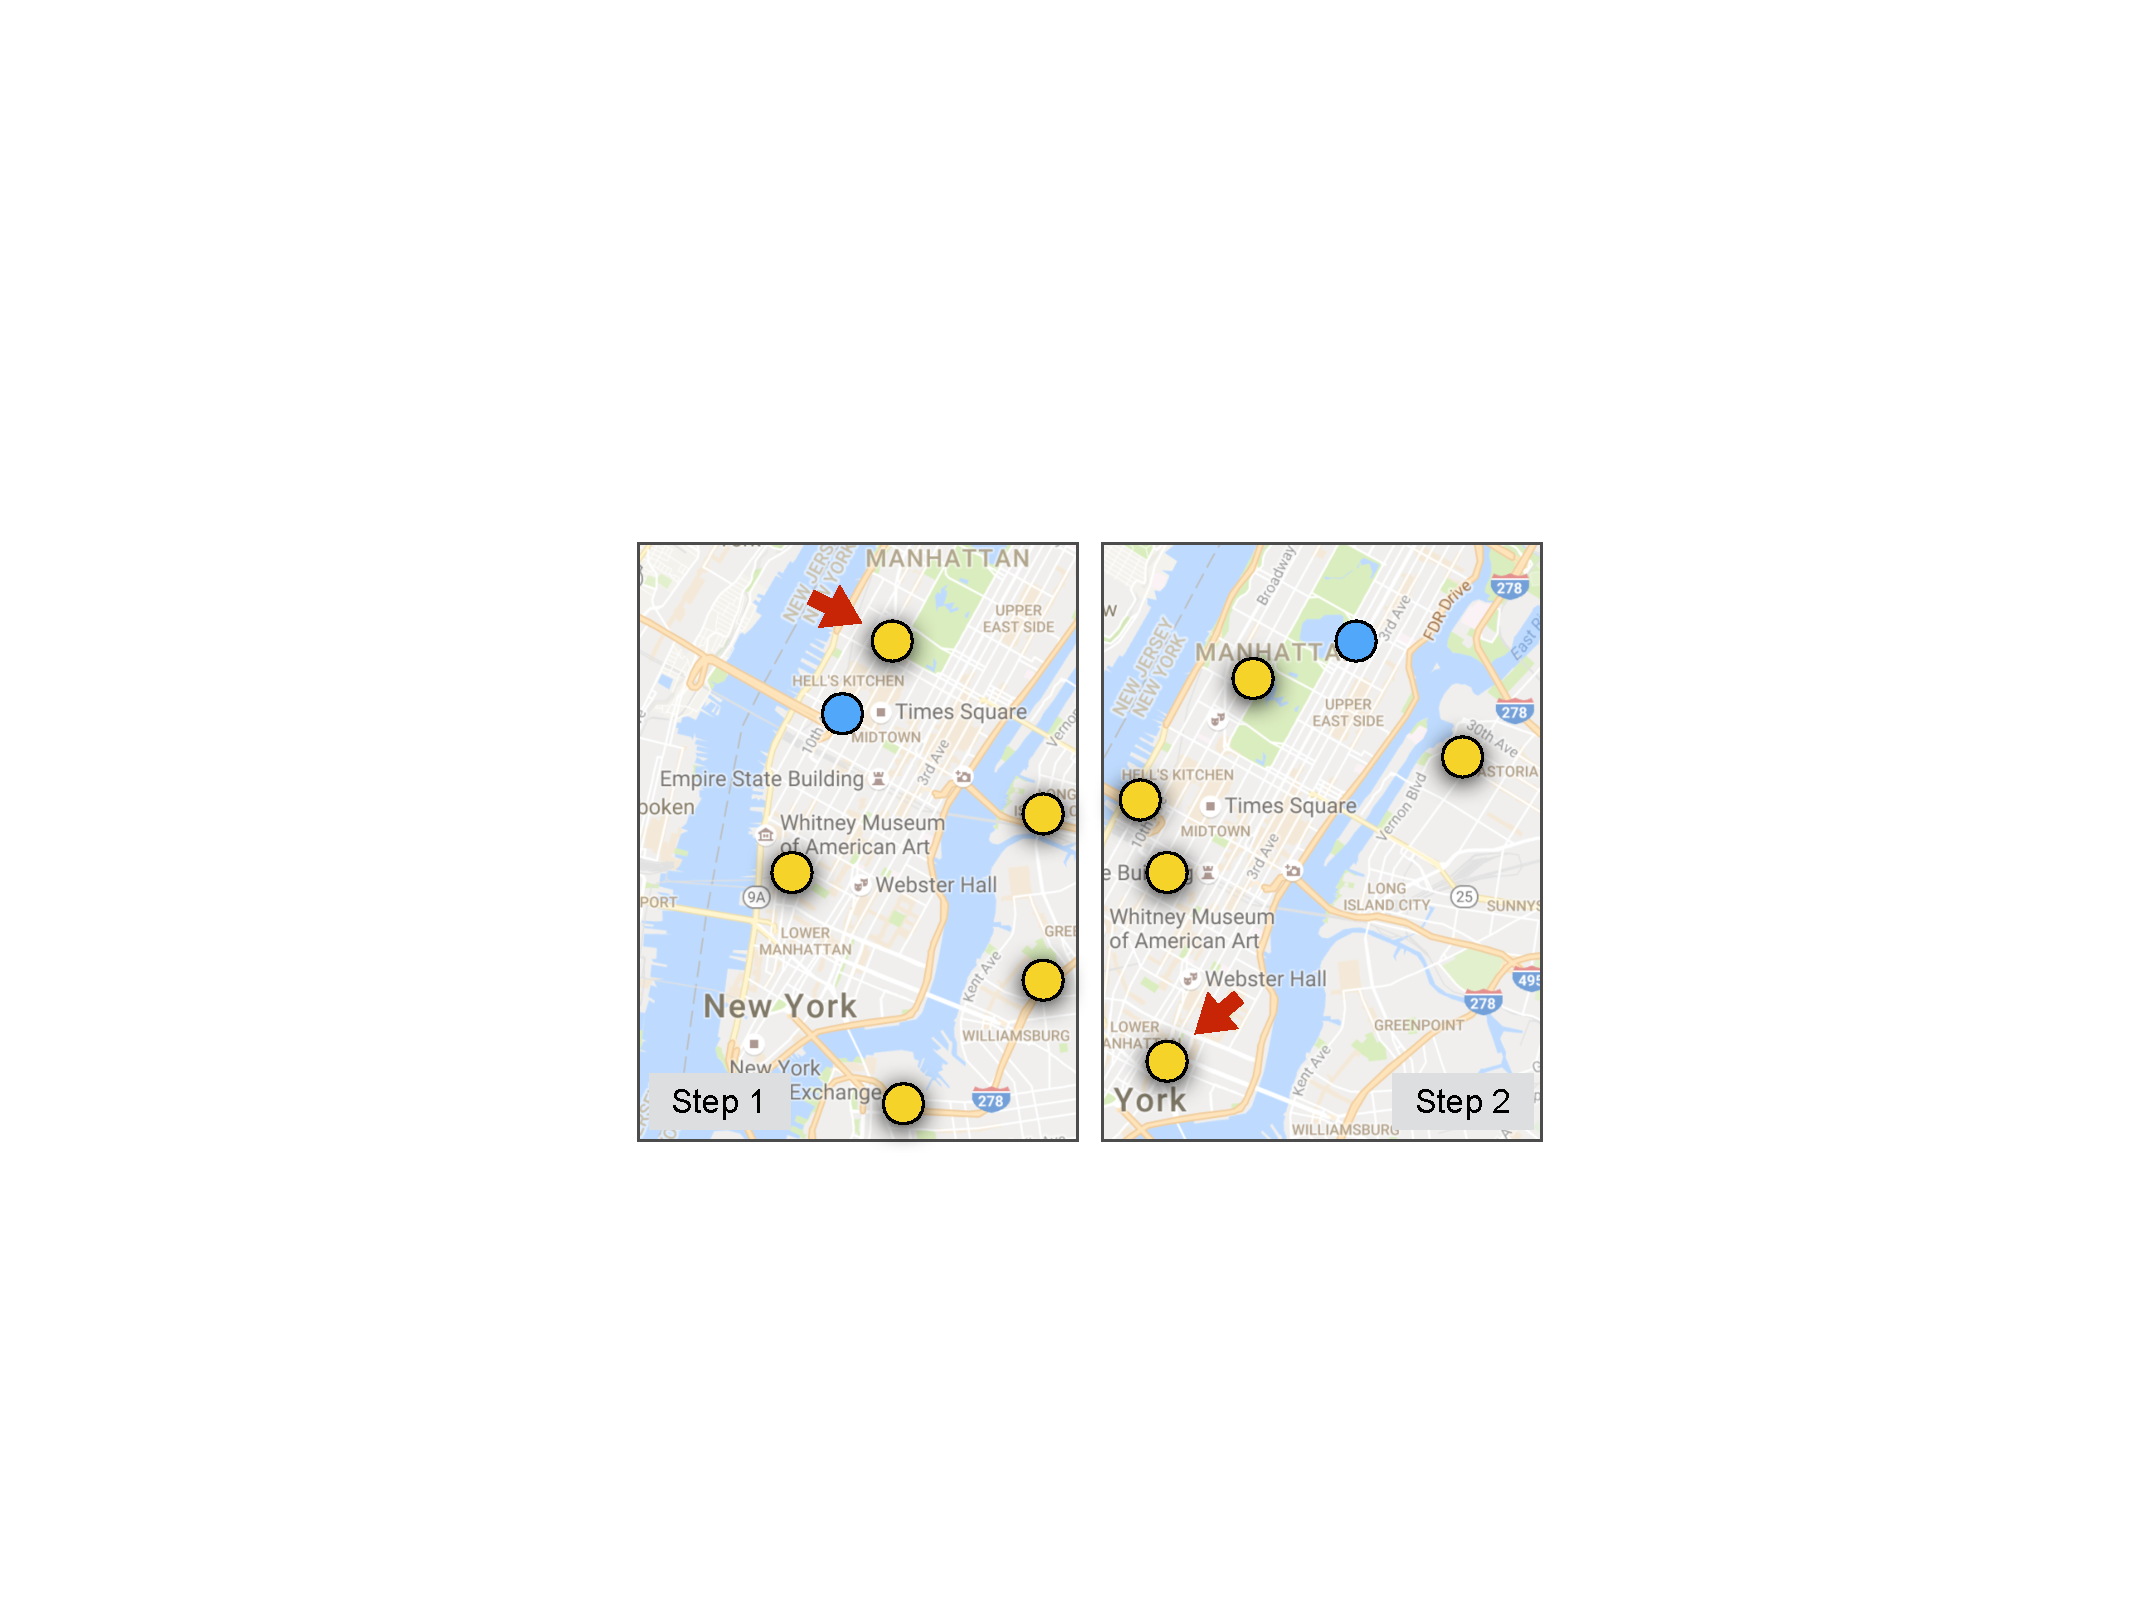
\includegraphics[width=\columnwidth]{figs/scn}
\caption{Application of \framework}
\label{fig:app}
\vspace{-10pt}
\end{figure}


% \vspace{5pt}
% Consider Lucas, a data scientist whose task is to optimize New York taxi trips. Focusing on cab-idle locations, he wants to discover which neighborhoods work the best for which drivers to increase the overall availability. Also, he wants to discover how drivers should choose their next cab-idle station to be more available. Lucas employs \framework\ and follows a case-by-case inspection as his analysis methodology by analyzing and learning from historical data.

% coordinates of first point picked: lat, long: 40.757555, -73.988832. Point ID-1274, equivalent to 270 W 43rd St, New York, NY 10036, EUA. Next to Times Square.
% coordinates of the second point: lat, long: 40.789358,-73.970172000000005. Point ID-968, equivalent to Columbus Avenue, New York, NY, EUA.
%  coordinates of the third point: lat, long: 40.717531999999999,-74.010260000000002. Point ID-192, equivalent to 183 Duane Street, New York, NY 10013, EUA

% He begins the analysis by selecting a point from the most crowded region in New York, i.e., Times Square (Figure \ref{fig:app} left). The point depicts a drop-off at {\em ``3 Times Square, New York, NY''} on January 9, 2014 around 9PM (the blue point in the figure). {\sc Highlighter} then provides $5$ relevant points to the selected point (yellow points in the figure).
% These highlights show similar points to the selection in other neighborhoods of the region.
% Among 5 highlighted points, Lucas selects a pick-up at {\em ``West 53rd Street''} near Central Park occurred approximately at the same time of the first selection (the point marked with an arrow in the figure). This pick-up has a potential to enchain with the first choice (i.e., a drop-off) to engage the driver in a larger distance.
% 
% In the next step, {\sc Highlighter} shows $5$ other points relevant to the new selection (Figure \ref{fig:app} right). Lucas looks for a good drop-off point which is in a neighborhood of the previous selection as the cab-idle station. Lucas selects a highlight in downtown as others are around the train station which have often less taxi requests at nights. This selection contributes to the heavy cab request in Manhattan island at that time of the day. Note that in both steps, the $k$ results are a compromise between relevance and diversity.

% The result of similarity for all two executions of the algorithm for the Lucas problem, considering $k = 5$ and $\sigma = 0.2$, was approximately, \textit{0.72}.

\bibliographystyle{abbrv}
\bibliography{main}

\end{document}
 
